\documentclass{article}
\usepackage{amsmath}
\usepackage{epsfig}
\usepackage[all]{xy}
\usepackage{multicol}
\usepackage{indentfirst}
\usepackage{algorithm}
\usepackage{algorithmic}
\setlength{\textwidth}{6.5in}
\setlength{\textheight}{9.5in}
\setlength{\topmargin}{0in}
\setlength{\oddsidemargin}{0in}
\setlength{\evensidemargin}{0in}
\setlength{\topmargin}{0in}
\setlength{\headheight}{0in}
\setlength{\headsep}{0in}
\setlength{\topskip}{0.5in}
\begin{document}
%% be sure to change the:
% Section number, Day, and time
% Date and year
% Name
% spellcheck using ``aspell -c filename'' in Unix
\begin{center}
\LARGE{\bf Parallelizing a Network Simulator}
%% PUT IN YOUR SECTION, DAY, AND TIME
%%example:
%% Section 7 - Thursday 8:30 AM\\

%% PUT IN THE DATE AND YEAR THE ASSIGNMENT IS DUE
%%example:
%% September 10, 2004
%% PUT IN YOUR NAME
\begin{center}
\Large{
Michael Bauer \hspace{1in} Nan Jiang
}
\end{center}
\Large{Department of Computer Science \\ Stanford University \\ \{mebauer, njiang37 \}@stanford.edu}
\end{center}

\begin{multicols}{2}
\begin{center}
\Large{\bf Abstract}
\end{center}
%\small{
\emph{In the context of the current multicore revolution, the need to
design an effective interconnect network has become increasingly
vital.  Computer architects make use of network simulators in order to
determine the best network designs and configurations.  The process by which this
is done however is often computationally intensive and requires
significant run time.  The fact that most simulators are single threaded
only adds to the computational bottleneck and renders them unable to take
advantage of new multicore processors.  This paper demonstrates how
an interconnect network simulator can be parallelized into a multithreaded
implementation.  The additional
performance gain from this parallel simulator ultimately can lead to decreased
development time and better designs as architects can sweep additional
parameter spaces and consider more configurations.}
%}
\section{Introduction}
After hitting the frequency and power walls, chip manufacturers have begun
to design and produce multicore chips that are capable of executing
multithreaded programs.  While this has greatly increased the computation power of the processors, existing programs that have been
written in a single threaded programming model must be rewritten in a
parallel programming model in order to take advantage of the additional cores.  This process of converting a program from a single threaded
programming model to a parallel programming model is a non-trivial task
that often requires restructuring the algorithm of the program as well as
how the data is organized and partitioned.  In this paper we demonstrate
several parallelization techniques in the process of parallelizing a
network simulator.\\
~\\
Another major ramification of the multicore revolution has been the
increased importance of interconnect network design.  As the number of
cores being placed on a chip increases, the processor interconnect plays a bigger and
bigger role in minimizing the latency of communication between processors
and providing enough bandwidth to allow for the movement of large chunks
of data. Traditional bus architecture is no longer the appropriate medium of communication for high number of core. Even more recent single crossbar communication hubs will also not be sufficient in the future, since the complexity of a single crossbar grows quadratically with the number of cores. Interconnection network can provide the scalable and efficient communication
infrastructures for future multicore processors. \\
~\\
In order to make informed decisions in the process of designing
interconnect networks, computer architects make use of simulators to
observe the effect of different network configurations and parameters.  While
these simulations can provide valuable insight into the best designs, they
often require sweeping a large, multi-dimensional parameter space.  In
addition, each simulation requires that many thousands of cycles
of network operation to be simulated.  This demands a large number of computational
resources in order to fully explore the design space.\\
~\\
The network simulator that we employ in this papaer was originally written
in a single threaded programming model.  This made the simulator extremely
slow and a single simulation of just a few thousand cycles would take many
minutes of compute time.  In order to speed up the process of running
simulations we have parallelized this simulator by making it
multithreaded.  In section \ref{background} we provide some background on
the simulator and its mechanics.  In section \ref{para} we describe the
means by which we parallelized the simulator.  We then describe in section
\ref{results} the results that we obtained from our parallel
implementation.  After demonstrating our performance gain and its limiting
factors we discuss how additional performance could be gained in section
\ref{disc}.  Finally, in section \ref{conc} we conclude.

\section{Simulator Background \label{background}}

The interconnection network simulator, Booksim, was created by the Concurrent VLSI Architecture group (CVA) at Stanford to study network on chip and large scale computer systems. The simulator allows for a wide range of user customizations when constructing a network. The simulator supports a variety of network topologies, router micro-architectures, routing algorithms, traffic pattern, and simulation modes. The priority of the simulator is  to guarantee the correctness and accuracy of simulation, and as a result the simulator is implemented in a cycle-accurate fashion. Booksim has been used to generate results for many research publications \cite{cdragon,KimISCA07,PPIN}. 
\subsection{Simulator Organization}
Booksim is written in C++ and dynamically allocates a hierarchy of objects to represent the user specified network. Figure~\ref{fig:simulator} shows the anatomy of the simulator at runtime. At the core of every network simulation is a collection of router and channel objects which forms the framework of a network. Each channel acts as a FIFO with a reader and a writer router object. The router objects contain all the data structure and operations necessary to route packets through the network. Similar to networks in real life, routers are mostly isolated from each other and can only communicate through the channels or simple global signals. As a result, the operations of individual routers are almost completely independent of other routers in the network. Surrounding the core network framework is the traffic manager which acts as an interface between the user tests and the underlying network. It handles the injection and ejection of traffic as well as gathering simulations statistics for the user. \\
~\\
\begin{figure}[h]
\centering
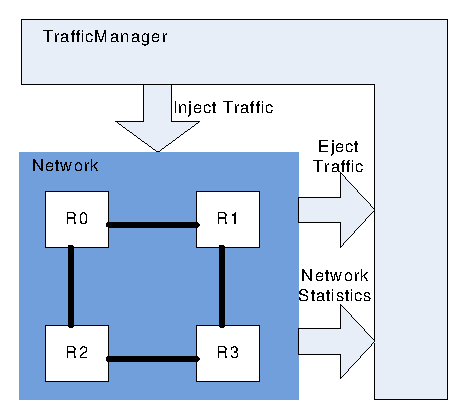
\includegraphics[width=3in]{simulator.eps}
\caption{Simulator organization: Network is composed of routers and channels and simulations are run through the traffic manager. }
\label{fig:simulator}
\end{figure}
Figure~\ref{fig:runtime} diagrams the runtime steps of the simulator. At the highest level is the network cycle loop. Each iteration of this loop represents a cycle in the network. Within each network cycle, several steps occurs to advance the state of the network. At each step, the simulator loops through all the routers in the network to perform a specific function. As mentioned previously the operation of routers are mostly independent of each other. Therefore, there are no dependencies between each iterations of these loops. Channels are the only source of sharing between the routers 
\begin{figure}[h]
\centering
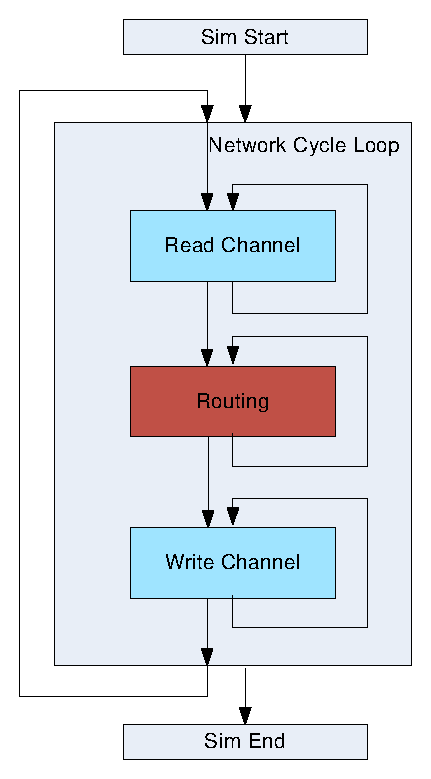
\includegraphics[width=3in]{runtime.eps}
\caption{Simulator runtime diagram. The number of iterations of the outer loop is equal to the number of simulated cycles. The number of iterations of each of the inner loops is equal the number of routers in the network.}
\label{fig:runtime}
\end{figure}
\subsection{Simulator Performance}
The simulator was originally designed for studying numerous aspects of small to medium sized interconnection networks (less than 100 network nodes). Nearly every aspect of the network is customizable and has been modeled in detail. Performance has not been a concern. However, the group's recent project involves simulating the dragonfly network \cite{cdragon}, which can easily grow to thousands or tens of thousands of nodes. Due to the organization of the simulator, the simulation runtime grows linearly with the number of network nodes and the number of simulated cycles. A typical simulation of the dragonfly network involves running a networks with 10K nodes for at least 10K cycles to capture the network's steady state. Under the current simulator, this takes about 25 minutes. To generate an accurate latency-throughput plot of the network requires about 10 simulations. Furthermore, to see the effect of changes to a particular aspect of the network requires generating a latency-throughput plot each time. Such long simulation time increase the turn around time for research and limits the number of experiments that can be run reasonably. Currently, the group utilizes program level parallelism by running multiple simulations simultaneously on a cluster. But they are still limited by the runtime of each simulation.

Previously we have profiled the simulator to determine the program characteristics and hotspots. The program is composed of mostly integer operations. The only sources of floating calculation are for random packet generation and statistics collection. The program is control flow intensive: there are numerous branches inside of long running loops to determine the flow of packets and state of the routers. The program is also relatively memory demanding, since each network component is created as an object and network packets objects are dynamically allocated and deallocated as they enter and exit the network. In the typical dragonfly network modeled with realistic channel latencies, there is potentially hundreds of thousands of packets in flight simultaneously. Runtime profiling shows that 95\% of program time is spent in the routing step in figure~\ref{fig:runtime}. 



\section{Parallel Implementation \label{para}}
In order to parallelize the network simulator, we first set about
identifying sources of parallelism that we could exploit.  As mentioned previous, the routers in a network operate relatively autonomously.   Each router in the network can be simulated
independently as long as the communication that occurs between the routers
is synchronized in the channels.  In this section we describe how we
partitioned the work of the network simulator and the synchronization
mechanisms that we employed in order to maintain the correctness of the simulator.

\subsection{Partitioning the Network}
The first step in parallelizing the simulator was to define a division of
work that could be spread across parallel threads with minimal amounts of
communication overhead.  Fortunately, the network simulator naturally
lends itself to this sort of partition in the sense that each router
within the network can be simulated almost entirely independent of every
other router.  In addition to this communication only occurs at the
beginning and end of every cycle of simulation when flits are either
written or read from the shared channels.  The significant
calculation of the arbitration logic is a much larger computational that
can be performed in an entirely local manner.  While this provided us with
a simple partition of work, it left us with several important issues both
for correctness and performance.

\subsubsection{Locking Channels}
We initially assigned routers to threads by their ID numbers which are completely independent of
topology.  This left us no easy way of determining which channels would
ultimately be shared and which would be local to a thread, therefore we
were forced to place locks on all channels to ensure correctness.  Since
the channels were initially represented as STL queues, there was no way to
allow concurrent accesses to the queues (i.e. we couldn't allow one router
to be reading and another to be writing simultaneously).  In order to
prevent this, we protected each queue with a Pthread lock.  For a thread
to access the queue, it first had to acquire the lock and then release the
lock when finished performing its operation on the queue.\\
~\\
While this approach guaranteed correctness, it also caused significant
performance overhead.  Even queues that were not shared between different
threads were having to be locked and unlocked in order to perform
operations on the queues.  In order to get around this additional
overhead, we instead began to partition the router work based upon the
topology of the network.  This therefore allowed us to know which channels
were shared and which were local to a single thread.  By doing this, we
were able to remove some of the overhead of locking when performing
operations on a channel's queue. However, this method adds an additional layer of complexity for the user. For each topology in the simulator, we need to write a network partitioning algorithm for that topology. Ideally we would like a generalized algorithm that would discover the optimal partitioning to minimize locking given any network. But this is not part of the scope of this project and has not been done. (***LOL NP COMPLETE??)

\subsubsection{Barriering Every Cycle}
While the difficulty of efficiently partitioning the network created
several performance issues, we also had to address the issue of the
correctness of the simulation.  By allowing each thread to operate
independently, we had created the potential for one or more threads to run
ahead of other threads in the simulation.  This means that different
threads could be performing computation on different cycles of the
simulation at the same time.  If not handled correctly, this could have
led to a correctness issue.  Consider the following example: assume that
one thread is simulating one cycle ahead of all of the other threads and the network channel latency is also one cycle.  In
order for this thread to execute, it first reads in all the flits that are
in its input channels.  However, all the other threads have yet to write
to their output channels from the previous cycle.  Therefore when the thread running ahead
performs its reads, it will observe that all its input channels are empty
and assume this is correct, when in reality, the flits simply have not
been written from the previous simulation cycle.\\
~\\
In order to successfully solve this data race, we initially place a
barrier after every cycle of the simulation.  This then mandated that
after a thread simulates a cycle, it must wait for all the other threads
in the simulator to reach the same point.  This ensures that all flits are
written into their proper channels before any thread attempts to read them
out when simulating the next cycle.  While this guarantees correctness, it
can add significant
synchronization overhead. Transient load imbalances in the network may occur even under uniform random traffic pattern, this will the cause some threads to run slower temporarily. The barrier will amplify these transient load imbalance since the simulator will run as fast as the slowest thread. In the next section we describe how we were
able to remove the barrier and the locks around the queues in order to
improve concurrency and minimize synchronization overheads.

\subsection{Lock-Free Queues}
In order to improve the concurrency of our network simulator, we decided
to incorporate the lock-free queues described in \cite{LF}.  The advantage
that these queues provide is that they allow multiple readers and writers
to the queue simultaneously.  While our simulator only requires that we
be able to have one reader and one writer, simultaneously, these queues
still allow us to remove any lock overhead from the simulation.  For
completeness we give a brief overview the implementation of lock-free
queues.

\subsubsection{Implementation}
Lock-free queues are based on the universal concurrent access algorithm
\cite{LF} that assumes that any access to the shared data structure can
see the data structure in any potential partially updated state.  The
algorithm then allows for the access to either help other accesses to
complete before actually completing itself.  While this may sound
conceptually simple, the combinatorial number of states of the data
structure and different readers and writers is astounding.\\
~\\
The lock-free queue implementation that we use begins by having a sentinel
at the head of the queue whose value is meaningless.  This eases some of
the implementation details of the queue.  Initially both the head and tail
pointers of the queue point to the sentinel.  Whenever a new item is added
to the queue, the tail pointer is moved to point to the end of the list.
Whenever an item is popped from the queue, the head is moved to point to
the new sentinel, the next item in the list.  In this case the old
sentinel can then be reclaimed.  Each element in the lock-free queue is
wrapped in an AtomicReference object.  This object ensures that the any
items in the queue can only be written to atomically.  A diagram of how
this works can be seen in Figure (need figure here).\\
~\\
We initially implemented this AtomicReference object with a Pthread
lock.  While this provided a finer granularity of access to shared
objects than previously, we realized that the overhead in the number of
locks was tremendous.  Instead we relied upon an extension to GCC 4.1.2
(need citation) that provided an atomic \_\_compare\_and\_exchange operation.
This operation was significantly less costly in terms of synchronization
overhead and was also much faster.\\
~\\
After testing our lock-free queues, we replaced all of
the queues in the simulator with our new queue implementation.  While this
proved fairly straight forward, we didn't initially account for the high
overhead that the lock-free queues themselves created.  The lock-free
queues involve the creation of multiple objects and accessing the
lock-free queues involves chasing many pointers through these structures
as well as rearranging many pointers.  In some cases this overhead proved
to be extreme.  In order to remove it, we created a common interface that
was shared between the lock-free queues and the STL queue.  This then
allowed us to create dynamic instances of either a shared queue or an STL
queue depending on whether the channel was shared.  This significantly
improved our performance as we will demonstrate in the section \ref{results}.

\subsubsection{Guaranteeing Correctness Without a Barrier}
After adding the lock-free queues to our implementation, we realized that
they would provide little benefit if the barrier were not also removed to
allow threads to run ahead.  In order to remove the barrier, we had to add
an additional piece of data to each shared queue: a semaphore.  This
semaphore would be used in the following way: anytime a write operation
occurred to the queue, an up operation was performed.  Similarly, anytime
a pop operation occurred to the queue, a down operation would have to be
performed first.  We also modified the routers such that for every cycle
of simulation, they would at perform at least one up operation on every
channel that they shared with another thread even if they didn't actually
write any flits to that channel.  Note that a down operation is not able
to proceed if the semaphore equals zero, implying that no router can ever
run ahead of any of its input queues.  By adding this feature to our
lock-free queues we were able to guarantee correctness in the simulator
without a barrier operation.  This greatly increased the amount of
concurrency present in the simulation by allowing different threads to be
simulating different cycles simultaneously.

\subsection{Fusing Loops}
The last operation that we performed on our code was to the inner loops in figure~\ref{fig:runtime} together.  The initial simulator implementation was written to make it
easy to understand the code and not for performance.  We moved all these operations into a single
'for' loop in order to help improve some of the temporal locality of the
code.  Not surprisingly this operation allowed the system to take
advantage of the cache hierarchy and provide additional performance gain.

\section{Results \label{results}}
Having completed a parallel implementation of our network simulator, our
next step was to analyze the performance of the simulator to determine how
much speedup it achieved.  We began first by analyzing the performance of
the different synchronization mechanisms to ensure that they held with our
hypotheses about which method permitted the most concurrency.  We then analyzed
our results on a series of architectures to determine the scalability of
the simulator as well as any potential bottlenecks.

\subsection{Analyzing Synchronization Mechanisms}
The first step in analyzing our parallelized network simulator was to
determine the performance of the different synchronization mechanisms that
we had employed at different points in development.  Figure \ref{synch}
shows the performance of the various synchronization mechansims on a
single node of the Hotbox cluster that consists of two Intel Xeon Quad
cores.  We only ran experiments up to 8 threads as this is the maximum
number of hardware thread contexts available without encountering the
overhead of using ethernet to communicate between nodes.\\
\begin{center}
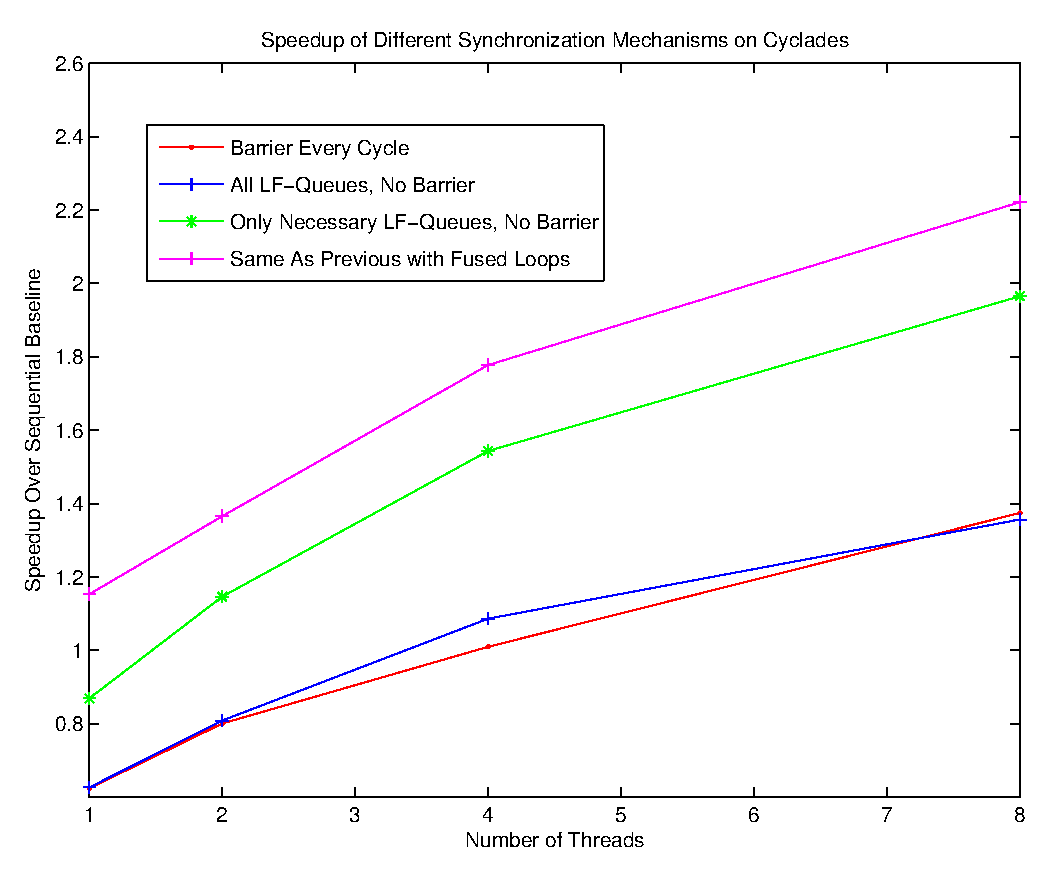
\includegraphics[width=3in,height=3in]{synch.eps} \\
\small{Figure 1: This figure shows the performance of the different
synchronization mechanisms on up to eight threads.}
\end{center}
From these results we can see that our hypotheses were confirmed regarding
the performance of the various synchronization mechanisms.  Barriering
every cycle added significant overhead to performance and ultimately
prevented even 8 threads from extracting much parallelism at all.
Surprisingly the same result was discovered when the barrier was removed and
all the queues were replaced with lock-free queues.  However, once we were
able to only implement the shared channels with lock-free queues , we could see a noticeable performance gain and even some
additional scalability.  Finally, once we fused several of the loops being
executed within the program, we were able to improve some of the temporal
locality of data use and thereby achieve a little additional
performance.\\
~\\
Despite our efforts however, we were only able to extract a two fold
speedup using eight threads, far below a linear speedup.  This was very
perplexing to us as we had consciously attempted to break up the work into
parallel computations that required very little inter-thread
communication.  In order to determine exactly what was causing us to lose
performance we then proceeded to run several experiments to find the
bottlenecks in the program.

\subsection{Determining Scalability Bottlenecks}
Having observed the somewhat poor performance of our application we then
set about attempting to determine the reason for such poor performance.
Our initial hypothesis was that application was memory bound based on the
fact that there is a significant amount of data being processed in our
simulator.  In addition to this, the fact that Pthreads is a shared memory
programming model implies that if the working set cannot fit inside the L2
cache, then there will be a significant amount of data being moved both to
and from main memory.\\
~\\
To test our hypothesis that the simulator was memory bound, we ran the
simulator again on the Hotbox cluster, but this time ran each thread on a
different node.  This allowed each thread to have access to the entire
memory bandwidth of its node, and in effect, thereby increase the total
amount of memory bandwidth available to the entire application.  The
results of this experiment can be seen in Figure \ref{smp}.\\
\begin{center}
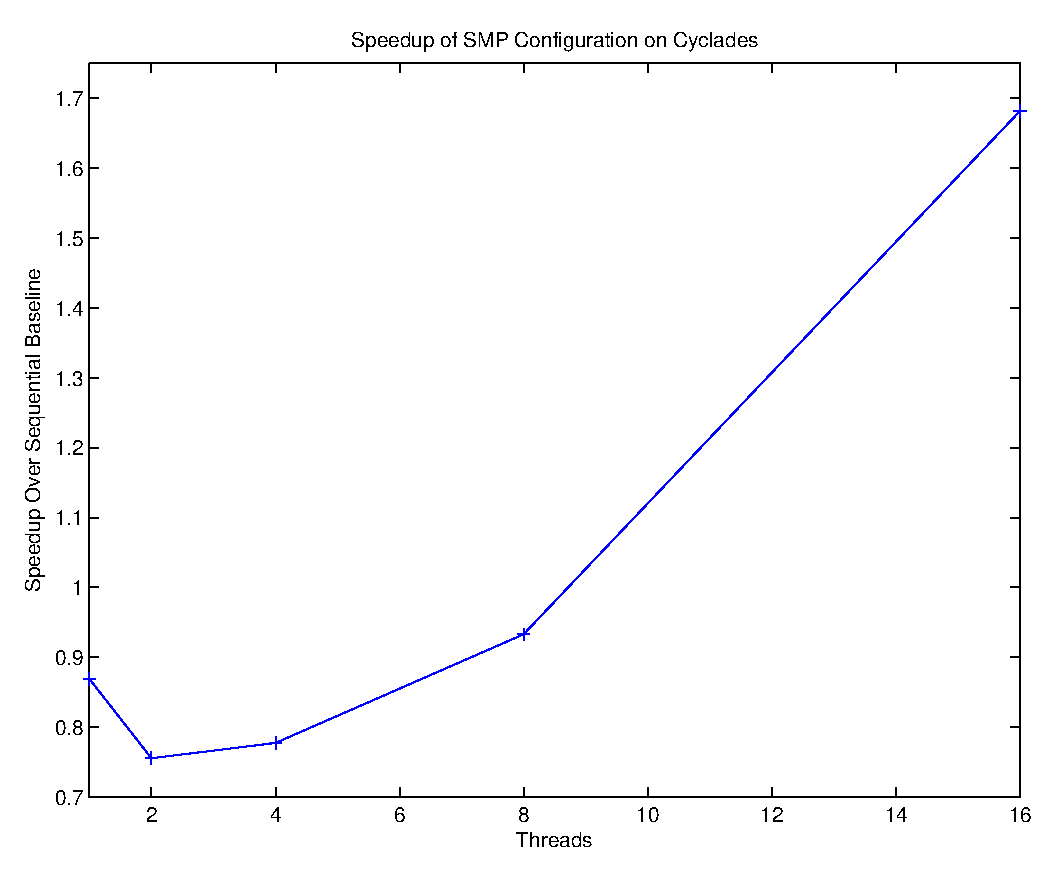
\includegraphics[height=3in,width=3in]{smp.eps} \\
\small{Figure 2: This figure shows the performance of the simulator on
up to 16 threads on a simulated SMP machine.  The speedup is relative to
the sequential simulator.}
\end{center}
From the result of this experiment we were able to see that bandwidth was
not the primary issue.  This is due to the fact that the performance of
the simulator remained poor and was even worse than the CMP version up to
16 threads.  In addition to revealing that the poor performance was not
due to memory bandwidth, it also revealed that communication was playing a
large role in the performance as the increased cost of communicating via
ethernet between nodes caused performance to be even worse than the CMP
configuration.\\
~\\
After realizing that our program was not memory bound, we wanted to see if
the size of the problem had any effect on the speedup.  We tested this by
plotting the speedup of a four threaded run on a given network size over the
sequential time for simulating the same size network on the Hotbox
cluster.  The results can be seen in Figure \ref{probsize}.
\begin{center}
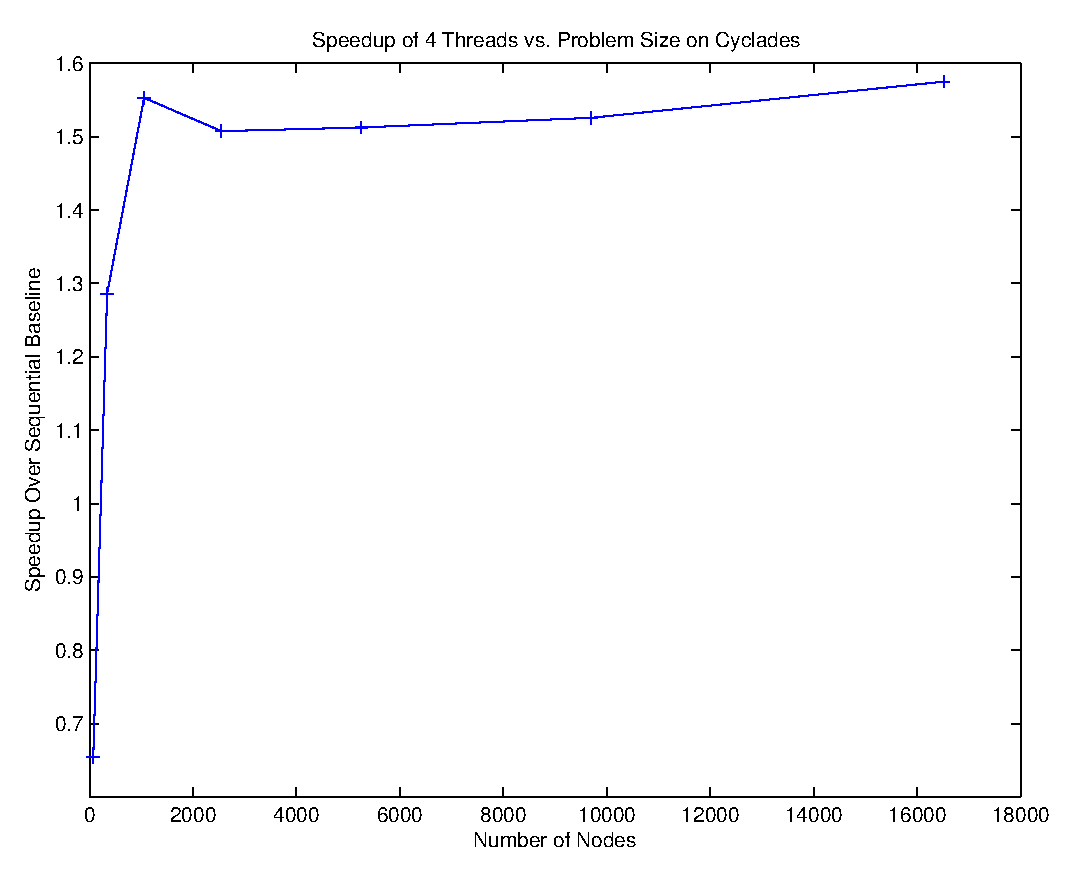
\includegraphics[height=3in,width=3in]{probsize.eps}
\small{Figure 3: This figure shows the speedup versus network size of a
four threaded run of the parallel simulator on the Hotbox cluster.}
\end{center}
From this figure we could see that essentially the speedup was independent
of problem size.  This meant that regardless of the size of the network
simulated, the four-threaded version ultimately was constrained by the
same relative to the sequential version.  The fact that the speedup
attained was significantly less than a linear speedup of 4 indicated that
the threads were not compute bound.  Instead we hypothesized that false
sharing was causing the four threads to thrash each others' caches.\\
~\\
To confirm our diagnosis of false sharing, we decided to run the simulator
on the both the Niagara T2 and T2+ machines.  Since these machines were
better designed to deal with long latency loads and stores, our hope was
that they would be able to mitigate the effects of false sharing to some
extend.  The results from this experiment can be seen in figure
\ref{niagara}.
\begin{center}
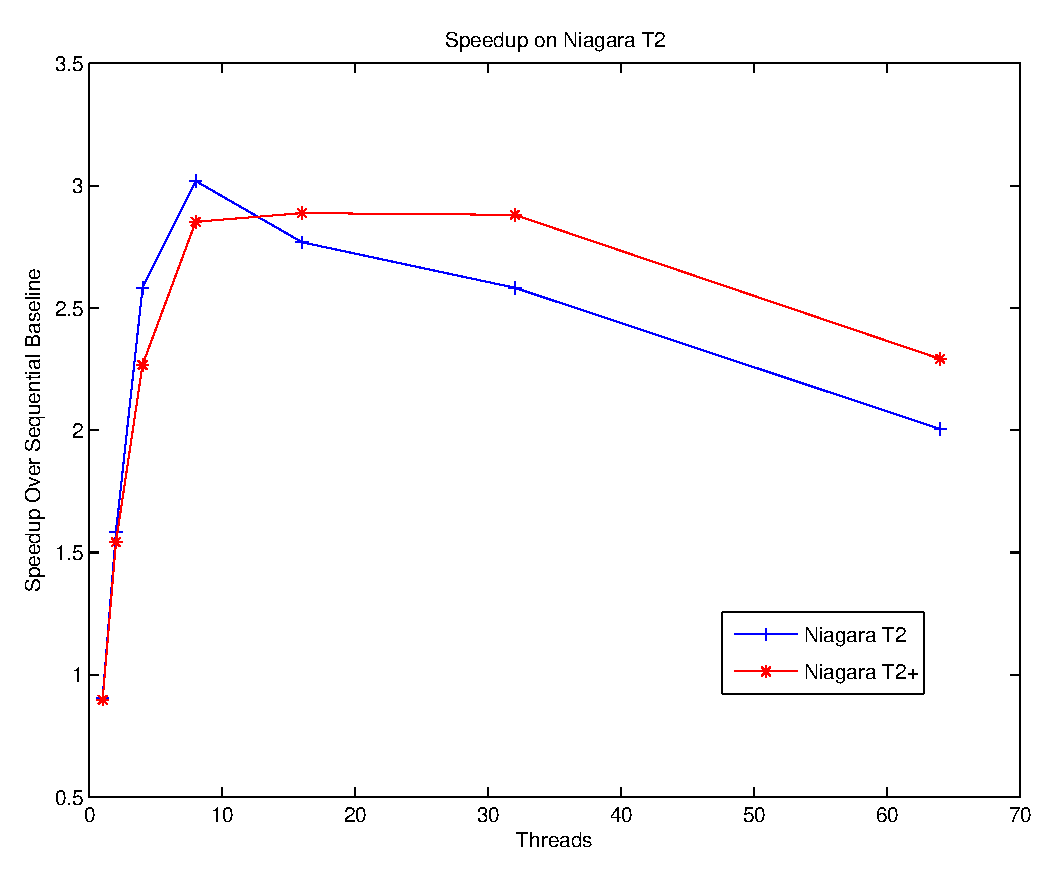
\includegraphics[height=3in,width=3in]{niagara.eps}
\small{Figure 4: This figure shows the speedup of the parallel simulator
up to 64 threads on the Niagara T2 and T2+ machines.}
\end{center}
We noticed that in this experiment, both the T2 and T2+ were able to
achieve some speedup to a certain number of threads, but then performance
began to fall off.  We determined that once the threads' working set sizes
began to interfere with each other in the shared L2 cache is when the
performance begins to degrade and couldn't offer us much insight into  any potential false sharing that was occurring when run on other
hardware platforms.

\section{Discussion \label{disc}}


\subsection{Static Network Partition}
The current implementation divides the network into equal partitions among the threads and seeks to minimize computation. This organization works well when the traffic pattern is balanced across the partitions. However, hotspot traffic patterns which concentrate the packets into a particular section of the network will cause imbalances in the amount of work handled by each thread. Even with the shared channel semaphore and the removal of the cycle barrier, the lightly loaded threads will  always be stalled waiting for the hotspot threads. Fortunately, common network traffic patterns are balanced and network routing algorithm are usually designed to reduce hotspots and bottlenecks in the network. Nevertheless, it is not a guarantee that an equally partitioned network will give equal work to all threads. Therefore, future improvements for the simulator should include dynamic partitioning of the network among the threads. This can be implemented by changing the current loop based iteration of network components into a work queue based organization. A work queue can be created for each network partition and each queue entry record the network component to be operated on and the network cycle associated with the operation. After operating on a component, the component is reinserted into the queue and the associated cycle is incremented. Under this organization, threads that have stalled ahead can pull work from other threads' work queues and help to finish the work in other network time slices.  

\subsection{Programming Model}
Given the underwhelming speedup that we obtained through parallelization and the possibility of excessive false sharing in the program, this has lead us to think that PThreads is not the most appropriate programming model for this simulator. As we have stated through out the report, the only points of sharing between threads are the channels that bridge routers running under different threads. No other source of true sharing should exist in the simulator. But with the shared memory model of PThreads, false sharing due to the organization of data structure can easily occur. Since we know the exact points of data sharing and since the smart partitioning of the networks should keep the amount of inter-thread communication small, perhaps message passing programming models such as MPI could offer more scalability for the parallel simulator. Shared channel objects can be written on top of MPI's send and receive interfaces, and many packets can be bundled together to reduce messaging overhead. 


\section{Conclusion \label{conc}}
We have developed a parallelized version of a interconnect network
simulator that is capable of achieving some speedup on both CMP and SMP
machines.  We outlined the basics of the simulator and the various
techniques that we used in order to extract concurrency from the
simulator.  We then demonstrated the performance of our parallel simulator
on several different hardware platforms.  Investigations showed that the
simulator is prone to suffering from false sharing and extreme
communication overheads.  Despite these bottlenecks we were able to
achieve up to a 3X performance which can significantly lower the
simulation time required for running future experiments.

%\begin{thebibliography}{99}
%\bibitem{LF} Herlihy, Maurice and Shavit, Nir {\em The Art of Multiprocessor Programming.} 2008.


%\end{thebibliography}

\bibliographystyle{IEEEtran}
\bibliography{paper}
\end{multicols}

\end{document}
